\documentclass[10pt,a4paper]{article}
\usepackage[utf8]{inputenc}
\usepackage[francais]{babel}
\usepackage[T1]{fontenc}
\usepackage{amsmath}
\usepackage{amsfonts}
\usepackage{amssymb}
\usepackage{graphicx}
\usepackage{float}
\usepackage{array}
\usepackage[left=2cm,right=2cm,top=2cm,bottom=2cm]{geometry}
\usepackage[svgnames]{xcolor}
\usepackage{listings} \documentclass[10pt,a4paper]{article}
\usepackage[utf8]{inputenc}
\usepackage[francais]{babel}
\usepackage[T1]{fontenc}
\usepackage{amsmath}
\usepackage{amsfonts}
\usepackage{amssymb}
\usepackage{graphicx}
\usepackage{float}
\usepackage{caption}
\usepackage{subcaption}

\lstset{language=python,
frame=single,
    basicstyle=\small\ttfamily,
    stringstyle=\color{DarkGreen},
    otherkeywords={0,1,2,3,4,5,6,7,8,9},
    morekeywords={TRUE,FALSE},
    deletekeywords={data,frame,length,as,character},
    keywordstyle=\color{blue},
    commentstyle=\color{DarkGreen},
}

\setlength{\parindent}{0pt}

\begin{document}

\begin{titlepage}
    \centering
    \vspace*{5cm}
    {\Huge\textbf{\textcolor{DarkRed}{TP3 - Support Vector Machine (SVM)}}\par}
    \vspace{1cm}
    {\Large Kenewy Diallo\par}
    \vfill
    \textcolor{Gray}{Université de Montpellier\par}
    \vspace{0.8cm}
    \vspace*{3cm}
\end{titlepage}

\section*{\textcolor{DarkBlue}{Introduction}}
Ce TP a pour objectif de pratiquer les techniques de classification SVM en utilisant le package \texttt{scikit-learn}, basé sur la bibliothèque \texttt{libsvm}. Nous allons explorer comment ajuster les \textcolor{Red}{hyperparamètres} et les fonctions noyaux pour optimiser la flexibilité du modèle.

\medskip

 Les morceaux de code ainsi que mes ajouts sont insérés tout au long du rapport.




\section*{\textcolor{DarkGreen}{Partie 1 : SVM sans optimisation}}
\subsection*{Question 1 }
Nous avons d'abord séparé le jeu de données \texttt{iris} en deux parties, une pour l'entraînement et une pour les tests :

\begin{lstlisting}
X, y = shuffle(X, y)
X_train, X_test, y_train, y_test = train_test_split(X, y, train_size=0.5)
\end{lstlisting}



\begin{lstlisting}[language=Python, caption=Initialisation et entraînement du modèle SVM avec noyau linéaire]
# Initialisation du modèle SVM avec noyau linéaire
clf_linear = SVC(kernel='linear', C=1.0)

# Entraînement du modèle
clf_linear.fit(X_train, y_train)
\end{lstlisting}


Le modèle a bien appris à classifier les instances dans les données d'entraînement avec une précision de 72\%. Toutefois, il généralise avec une précision de 68,6\%, indiquant une légère sur-adaptation. Cela pourrait être amélioré en ajustant le paramètre $C$.

\begin{table}[h!]
    \centering
    \begin{tabular}{|c|c|}
        \hline
        \textbf{Données} & \textbf{Précision} \\
        \hline
        Entraînement & 72\% \\
        \hline
        Test & 68,6\% \\
        \hline
    \end{tabular}
    \caption{Précision du modèle sur les données d'entraînement et de test.}
\end{table}


\medskip
\subsection*{Question 2}
Nous nous retrouvons maintenant avec un score de 0.7 avec un noyau polynomial pour les données d'entraînement et un score de 0.76 pour les données de tests. C'est mieux que pour le noyau linéaire pour les données de tests mais moins bon pour les données d'entraînement.


\begin{figure}[h!]
    \centering
    \includegraphics[width=0.8\textwidth]{images/im2b.png}
    \caption{Comparaison entre un noyau linéaire et un noyau polynomial.}
\end{figure}


\section*{  Comparaison des noyaux}

Il est possible de comparer différents noyaux pour la classification. Ici, nous avons comparé un noyau linéaire avec un noyau polynomial de degrés 1, 2 et 3.

\begin{lstlisting}[language=Python, caption=Comparaison des noyaux linéaire et polynomial]

degrees = list(map(int, np.r_[1, 2, 3]))
# Définition du grid de paramètres
parameters = {'kernel': ['poly'], 'C': Cs, 'gamma': gammas, 'degree': degrees}
# Utilisation de GridSearchCV
clf_poly = GridSearchCV(SVC(), param_grid=parameters, n_jobs=-1)
clf_poly.fit(X_train, y_train)
\end{lstlisting}

On obtient ainsi les meilleurs paramètres :
\begin{itemize}
    \item C : 0.0316
    \item Degree : 1
    \item Gamma : 10.0
    \item Kernel : polynomial
\end{itemize}

Le polynome dégré 1 est le meilleur aprés validation croisée



\section*{\textcolor{DarkGreen}{Partie 3 : Influence du paramètre $C$}}
\subsection*{Question 3}
Nous avons étudié l'effet de la constante de régularisation \textcolor{Red}{$C$} sur l'accuracy du modèle. Voici les résultats obtenus pour différentes valeurs de $C$ :

\begin{table}[H]
\begin{tabular}{|l|*{6}{>{\centering\arraybackslash}p{2cm}|}}
\hline
\rule[-1ex]{0pt}{2.5ex} \textcolor{Red}{Valeur de $C$} & 1 & 0.1 & 0.01 & 0.001  \\
\hline
\rule[-1ex]{0pt}{2.5ex} \textcolor{Blue}{Accuracy} & 96 & 96 & 96 & 92  \\
\hline
\end{tabular}
\caption{\textcolor{DarkGreen}{Variation de l'accuracy en fonction de $C$.}}
\end{table}

\begin{figure}[H]
\begin{tabular}{ccc}
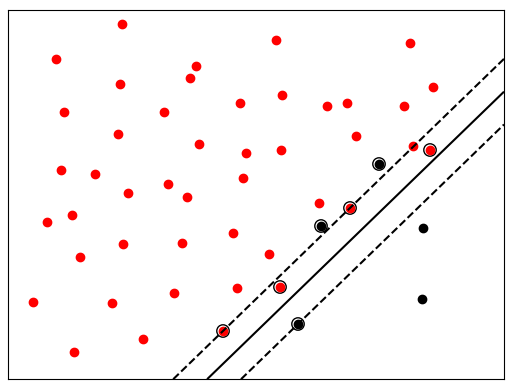
\includegraphics[width=0.33\linewidth]{images/libC1.png} & 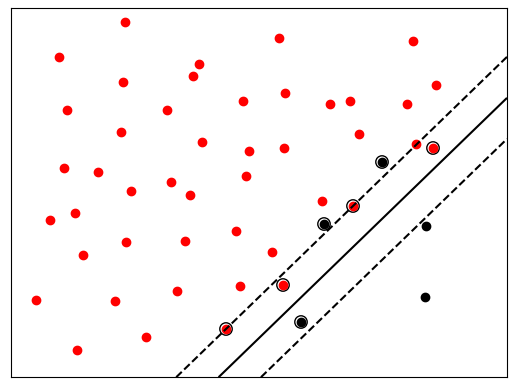
\includegraphics[width=0.33\linewidth]{images/libC0_1.png} & 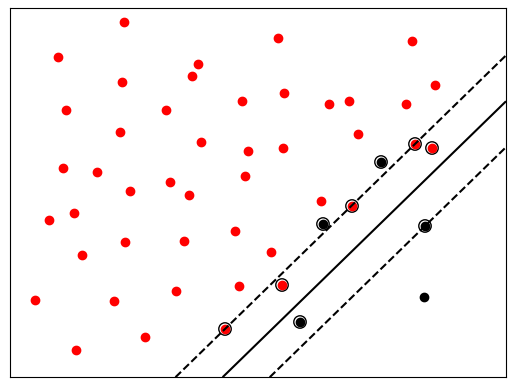
\includegraphics[width=0.33\linewidth]{images/libC0_01.png} \\

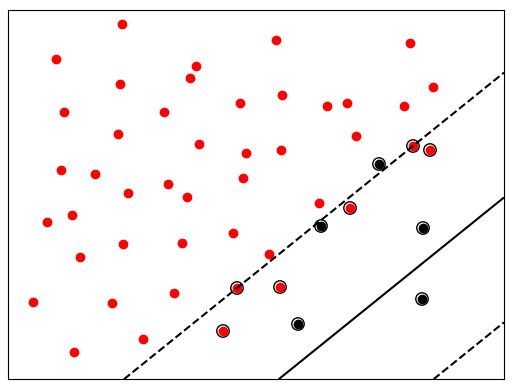
\includegraphics[width=0.33\linewidth]{images/libC0_001.png} &
\end{tabular}
\caption{\textcolor{DarkOrange}{Classification avec noyau linéaire pour différentes valeurs de $C$.}}
\end{figure}
On constate qu'en diminuant le paramètre \(C\), la marge se déplace jusqu'à devenir incorrecte. En effet, dans la dernière image, on remarque que des points noirs se situent dans la même région que les points rouges, ce qui induit une mauvaise classification.


\medskip
\section*{Question 4 : Classification de visages}

Le score d'apprentissage augmente avec la valeur de $C$ jusqu'à atteindre un palier à partir de $C = 10^{-3}$ que l'on va donc considérer comme notre meilleur paramètre.

\begin{lstlisting}[language=Python, caption=Fit d'un classifieur linéaire et test sur différentes valeurs de C]
Cs = 10. ** np.arange(-5, 6)
scores = []
for C in Cs:
    clf = SVC(kernel='linear', C=C)
    clf.fit(X_train, y_train)
    scores.append(clf.score(X_train, y_train))
\end{lstlisting}

\begin{figure}[h!]
    \centering
    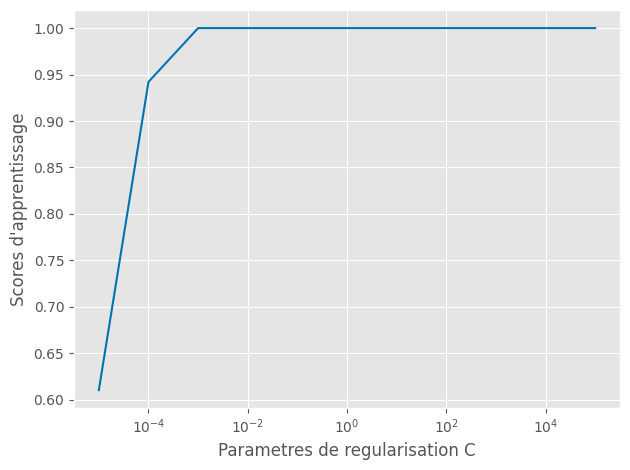
\includegraphics[width=0.8\textwidth]{images/IM7.png}
    \caption{Évolution du score en fonction du paramètre de régularisation $C$.}
\end{figure}

On obtient alors les résultats suivants pour la valeur de $C = 10^{-3}$ :
\begin{itemize}
    \item Niveau de chance : 0.6211
    \item Précision : 0.9105
\end{itemize}




\begin{lstlisting}[language=Python, caption=Prédiction des étiquettes pour les images de test]
clf = SVC(kernel='linear', C=Cs[ind])
clf.fit(X_train, y_train)
y_pred = clf.predict(X_test)
\end{lstlisting}

 On pourrait aussi tracer la courbe de l'erreur par validation croisée sur le paramètre C.
 
\begin{figure}[h!]
    \centering
    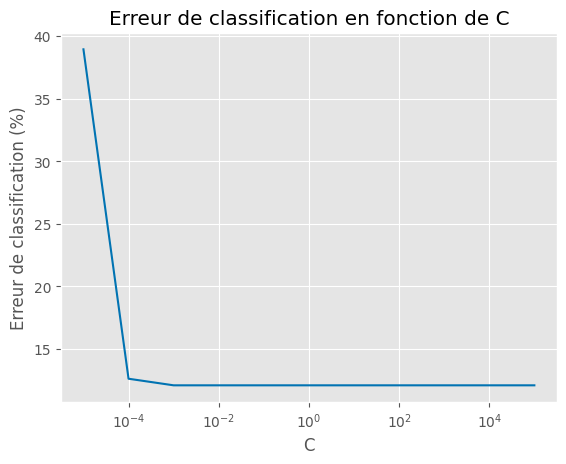
\includegraphics[width=0.8\textwidth]{images/IM8.png}
    \caption{Erreur de prédictions en fonction de $C$ obtenue par validation croisée.}
\end{figure}


\newpage  % Passe à une nouvelle page
\noindent On retrouve  la valeur de $C = 10^{-3}$ qui va minimiser l'erreur de prédiction.


\begin{lstlisting}[language=Python, caption=Courbe de l'erreur par validation croisée]
# courbe de l'erreur par cross validation
from sklearn.model_selection import cross_val_score
err = []
for C in Cs:
    clf = SVC(kernel='linear', C=C)
    scores = cross_val_score(clf, X_train, y_train, cv=5)
    err.append((1 - scores.mean()) * 100)
\end{lstlisting}


\newpage  % Passe à une nouvelle page
\noindent Et pour les images on'a :




\begin{figure}[h!]
    \centering
    \includegraphics[width=0.8\textwidth]{images/f.png}
    \caption{Prédiction entre Colin Powell et Tony Blair.}
\end{figure}

\newpage  % Passe à une nouvelle page
\noindent On observe en conséquence sur le jeu de données des images une erreur de une prédiction sur les 12 ce qui
correspond bien à une Accuracy de 0, 91.

\begin{figure}[h!]
    \centering
    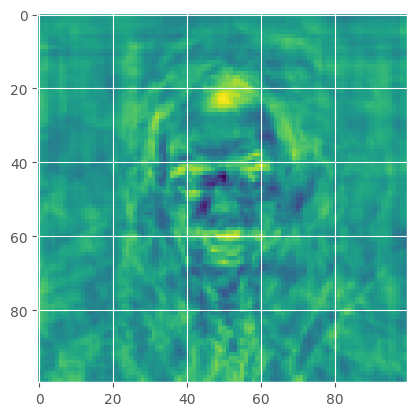
\includegraphics[width=0.8\textwidth]{images/IM11.png}
    \caption{Importance des différents pixels dans la décision.}
\end{figure}


Sur la figure 6, les pixels aux couleurs les plus vives, qu'elles soient claires ou foncées, se distinguent nettement. Ce sont ces pixels, représentant les variables, qui contribuent le plus à la prédiction lors de la classification.






\textbf{Question 5 : Introduction de bruit}

En introduisant du bruit suivant une loi normale centrée réduite sur notre échantillon, nous constatons que le score diminue drastiquement :

\begin{lstlisting}[language=Python, caption=Impact du bruit sur le score]
run_svm_cv(X, y)
run_svm_cv(X_noisy, y)
\end{lstlisting}

\begin{itemize}
    \item Score sans variable de nuisance : 0.9
    \item Score avec variable de nuisance : 0.5
\end{itemize}
 Nous ajoutons des variables de bruit au modèle pour évaluer l'impact sur ses performances. Sans nuisance, le score de généralisation est de 0.9 (moyenne de 10 simulations). Avec des variables de nuisance, le score chute à 0.54, indiquant une dégradation significative des performances. 


il peut etre represnte graphiquement 

 \begin{figure}[h!]
    \centering
    \includegraphics[width=0.8\textwidth]{images/sans ou avec.png}
    \caption{Évolution du score en fonction du paramètre de régularisation $C$.}
\end{figure}


\newpage\textbf{Question 6 : Réduction de dimensions}


Nous pouvons réduire les dimensions pour améliorer la prédiction en ajustant le paramètre ncAdhérents = 20. On applique ensuite l'ACP sur les données bruitées avec PCA(n_components=ncAdhérents, svd_solver="randomized"), puis on transforme les données bruitées avec pca.fit_transform(X_noisy)

il peut etre represente graphiquement 





\begin{figure}[H]
    \centering
    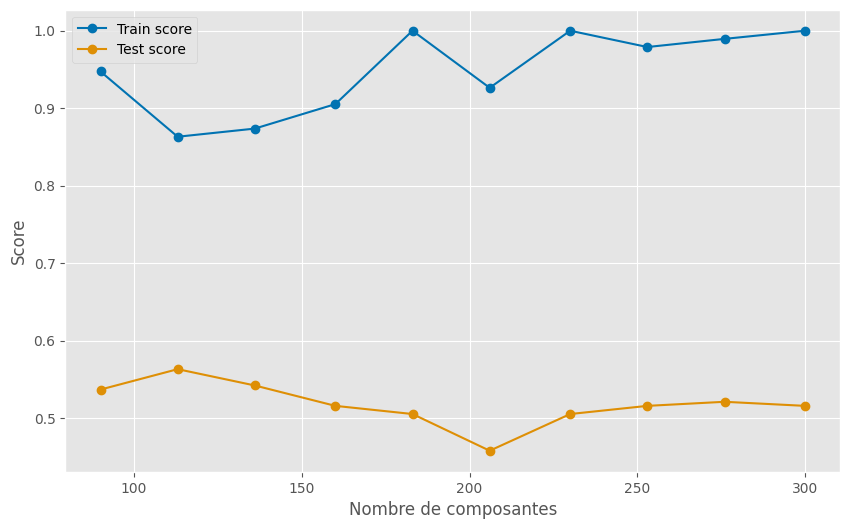
\includegraphics[width=0.7\linewidth]{images/graphPCA.png}
    \caption{Score en fonction du nombre de composantes de l'ACP}
    \label{fig:q6}
\end{figure}

Dans ce cas de figure on arrive pas tirer une ou des conclusions mais neamoins on peut utliser une autre methode c'st a dire calculer le score en jouant sur le nombre de paramétre 


\section*{Réduction de dimensions avec ACP}

En diminuant la dimension de l'espace de départ en cherchant les composantes principales par ACP, voici les résultats obtenus :

\begin{table}[h!]
    \centering
    \begin{tabular}{|c|c|c|c|}
        \hline
        \textbf{Nombre de composantes} & 5 & 10 & 20 \\
        \hline
        \textbf{Score d'apprentissage} & 0.6059 & 0.6043& 0.6570 \\
        \hline
        \textbf{Score de test} & 0.6153 & 0.6364& 0.5899 \\
        \hline
    \end{tabular}
    \caption{Scores d'apprentissage et de test pour des variables bruitées en fonction du nombre de composantes principales.}
\end{table}


\begin{lstlisting}[language=Python, caption=Réduction de dimensions avec ACP]
n_components = 20 # jouer avec ce parametre
print(f'Score apres reduction de dimension avec {n_components} composantes principales')
pca = PCA(n_components=n_components).fit(X_noisy)
X_pca = pca.transform(X_noisy)
run_svm_cv(X_pca, y)
\end{lstlisting}

L'erreur diminue avec certaines composantes principales, mais au-delà de certains rangs , elles semblent ajouter du bruit et dégradent le score. 
Faut noter qu'aussi ça demande un temps de calcul trés long (donc c'est a utitiser avec precaution )

\section*{Conclusion}

Ce travail pratique sur les Machines à Vecteurs de Support (SVM) a permis d'explorer différentes approches de classification supervisée en utilisant divers types de noyaux et des techniques d'optimisation des hyperparamètres, telles que la validation croisée. L'étude a montré l'efficacité des noyaux linéaires et polynomiaux, tout en soulignant l'importance du paramètre \( C \) dans l'équilibrage entre la précision du modèle et sa capacité de généralisation.

L'ajout de variables de nuisance a entraîné une diminution marquée des performances prédictives, ce qui a été partiellement compensé par l'utilisation de l'Analyse en Composantes Principales (ACP) pour réduire la dimensionnalité. Cependant, cette réduction des dimensions n'a pas totalement résolu le problème de sur-apprentissage, ce qui souligne la nécessité d'explorer d'autres méthodes plus adaptées aux données bruitées.





\end{document}


